\chapter{Características del sistema}

Dada las particularidades del problema a resolver, el sistema que se implementa está basado en el paradigma de la programación orientada a agentes para permitir la colaboración de los drones pertenecientes a la flota de exploración de manera eficiente. De esta manera la solución que se presenta está basada en la máquina de estados de la Figura 1, siendo la misma ejecutada por todos los drones de manera autónoma. 
La máquina de estados contempla la estrategia de exploración a utilizar, la definición del protocolo de comunicación entre los drones y el monitoreo del estado de la batería de cada dron.
En la siguiente sección se detalla el funcionamiento de la máquina de estados.

\begin{figure}[h!]
	\label{fig:comp}
	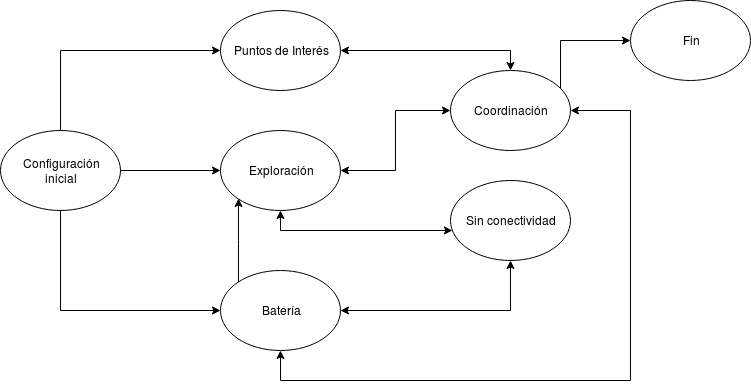
\includegraphics[width=.8\textwidth]{imagenes/chap5/image1}
	\caption{Máquina de estados simplificada.}
\end{figure}

\section{Máquina de Estados}
\subsection{Configuración inicial}

\begin{figure}[h!]
	\label{fig:comp}
	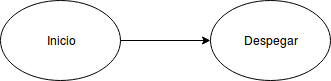
\includegraphics[width=.8\textwidth]{imagenes/chap5/image2}
	\caption{Especificación del estado Configuración inicial.}
\end{figure}

Al iniciar el sistema se realizan las configuraciones iniciales en el estado Inicio, donde se configuran las propiedades necesarias para la ejecución del sistema.
Es vital para el correcto funcionamiento del sistema establecer un canal de comunicación entre los drones que les permita intercambiar la información recabada a lo largo de la ejecución. La conexión entre los drones se implementa por medio de una arquitectura cliente-servidor, donde cada dron define al iniciar la ejecución del sistema un servidor TCP configurado para recibir la información de los demás drones y transmitirla a la máquina de estados. A su vez se define un cliente TCP para poder enviar los mensajes necesarios, siendo el mismo accesible desde los estados que requieran comunicarse con el resto de la flota
Existen varios propiedades parametrizables para la ejecución del sistema entre las que se incluyen:
las dimensiones del territorio a explorar 
las propiedades de la red wifi a la cual se conecta el dron
el tiempo total de ejecución del sistema
el algoritmo de exploración a utilizar
los puntos de interés a explorar
la altura a la que se mantiene el vuelo durante la exploración
activar funcionalidades complementarias como streaming de la exploración y el movimiento con rotación del dron
También se ejecuta un algoritmo de sincronización que permite a los drones comenzar la ejecución del resto de la máquina de estados al mismo tiempo. Esto permite que el tiempo de misión total de todos los drones sea el mismo y coordinar los tiempos en los que se deben visitar los puntos de interés.
Una vez concluida la etapa de inicio se procede al estado Despegar, donde se le envía al dron la instrucción de despegue y se determina cuál será el siguiente estado. 
\subsection {Exploración}

\begin{figure}[h!]
	\label{fig:comp}
	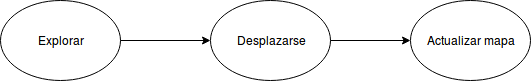
\includegraphics[width=.8\textwidth]{imagenes/chap5/image3}
	\caption{Especificación del estado Exploración.}
\end{figure}

La estrategia de exploración sigue el esquema de la Figura 3, donde se analiza para cada movimiento cuál es la nueva zona a visitar, consiguiendo de esta forma seguir un algoritmo que sea reactivo a la situación actual de la realidad tomando la mejor decisión en función de los datos recabados.
En el estado Explorar es donde se determina cual es el siguiente movimiento a realizar. Para calcular la próxima zona se cuenta con 2 alternativas, las cuales serán analizadas en la sección de experimentación para determinar cuál de ellas es más efectiva. Una de las alternativas diseñadas es utilizar un algoritmo greedy basado en determinar el siguiente movimiento en función de seleccionar entre las zonas vecinas, seleccionando aquella que fue visitada con mayor antelación o que nunca haya sido visitada. La otra opción es una variante del algoritmo descrito anteriormente, donde además se divide el territorio a explorar en diferentes regiones, por lo que al momento de determinar el siguiente movimiento no solo se consideran las zonas vecinas a la posición actual del dron, sino que también se realiza un control sobre el cubrimiento de las diferentes regiones del mapa determinando, en caso de ser necesario, desplazarse a una nueva región si la misma no cumple con las expectativas de la exploración.
Una vez determinado el siguiente movimiento a realizar se ejecuta el estado Desplazarse, donde se le envía al dron la instrucción de moverse hacia la posición calculada.
Al momento de finalizar el desplazamiento el dron cambia al estado Actualizar mapa, donde se registra la posición actual como visitada 

\subsection {Puntos de interés}

\begin{figure}[h!]
	\label{fig:comp}
	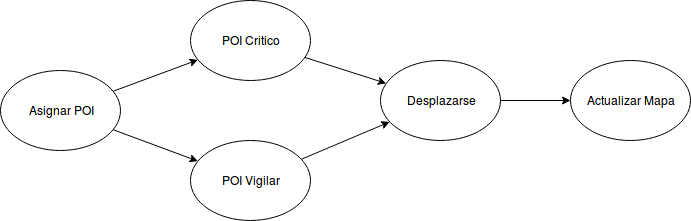
\includegraphics[width=.8\textwidth]{imagenes/chap5/image4}
	\caption{Especificación del estado Puntos de interés.}
\end{figure}

Cada punto de interés tiene un intervalo de tiempo asociado en el cual debe ser visitado por algún dron. En el caso de que no se cumpla con este requisito para algún punto de interés los drones entran en el estado Asignar POI, en el cual los drones eligen de forma conjunta a uno de ellos para que se encargue de ir a esa posición en forma prioritaria. Para tomar esta decisión los drones implementan un algoritmo de consenso basado en Paxos [27].



\subsubsection{Algoritmo de consenso}
Paxos es un algoritmo de consenso basado en el envío de mensajes que asegura un consenso entre N procesos participantes siempre y cuando se cumplan algunas condiciones:
La cantidad de procesos que fallan en algún momento del algoritmo no sea mayor o igual a N/2.
Los procesos pueden tener fallos pero no envían información incorrecta de forma intencional (no se producen fallos bizantinos).
Los procesos se envían mensajes asincrónicos que pueden tomar un tiempo indeterminado en llegar o directamente pueden perderse.
Si un mensaje llega a destino este no es corrupto, o si lo es se puede detectar.
Todos los procesos pueden enviarles mensajes a los demás de forma directa
Durante la ejecución del algoritmo no tiene porqué haber un proceso que actúe de líder, de hecho varios procesos pueden actuar como si fueran el líder, pero eventualmente se debe decidir un líder que dirima situaciones de conflicto.

En la implementación desarrollada del algoritmo todos los procesos actúan como líder hasta el final del proceso. Se define un líder solo en caso de que haya empates en la decisión final tomada y el líder se decide en base a la dirección IP de los drones: el dron que participa en el algoritmo que tenga el número más grande de IP es el líder. Se tomó esta decisión porque no todos los drones tienen porque participar en el algoritmo de consenso, solo lo hacen aquellos que se encuentren conectados a la red, tengan disponibilidad de batería y que no se encuentren en otra misión de alta prioridad. Esto lleva a que en cualquier ejecución del algoritmo de consenso pueda haber cualquier combinación de drones participando, por lo que se necesitaría un orden jerárquico completamente definido para establecer un líder desde el principio. Además los drones pueden perder conexión en cualquier momento del algoritmo, por lo que no resulta muy conveniente depender de que un único dron sea líder durante todo el proceso.

Además de la figura de líder, en un algoritmo Paxos se definen otros tres roles:
Proponentes: Son aquellos procesos que proponen valores para la decisión
Aceptadores: Son aquellos procesos que deciden aceptar o no los valores propuestos por los Proponentes
Receptores: Son aquellos procesos que no tomaron parte en el algoritmo de consenso y que deben ser informados de su resultado

La implementación propuesta hace que todos los drones participantes en la toma de decisión sean a la vez Proponentes y Aceptadores. De nuevo, esto se debe a que cualquier combinación de drones puede participar en el algoritmo y no existe un criterio objetivo para dictaminar quienes serán Proponentes o Aceptadores.

El algoritmo se divide en varias etapas:
Paso 1: Los drones que se encuentran disponibles (entendiéndose por disponible que tienen suficiente batería y no se encuentran realizando otras tareas prioritarias) le envían mensajes a todos los otros drones de la red informándoles de que quieren participar en la toma de decisión para el punto de interés correspondiente. Luego se quedan esperando durante un cierto tiempo configurable a que otros miembros de la red les envíen mensajes similares. De esta forma cada dron genera una lista con todos los drones participantes en la toma de decisión. Estos drones pasan a convertirse en los procesos participantes en la toma de decisión. Para evitar inconsistencias en la lista de participantes, la ventana de tiempo en la que los drones pueden mandar estos mensajes para participar se mide desde el momento en que el primer dron envía sus mensajes de participación. Esta técnica para sincronizar las ventanas de tiempo en las que se pueden enviar mensajes se usa en los otros pasos del algoritmo.
Paso 2: Una vez que se establece la lista de participantes todos los participantes se envían mensajes entre ellos informando de su distancia al punto de interés a atender. De nuevo, se establece una ventana de tiempo para la cual estos mensajes son válidos y que es absoluta para todos los drones.
Paso 3: Con la información obtenida en el paso 2 cada participante determina de forma independiente cual es el dron más cercano al punto de interés y envía un mensaje a los demás proponiendo a ese dron como candidato a vigilar el POI. Si existen dos drones que se encuentran a la misma distancia se elige al que tenga mayor valor de IP. Como siempre, se establece una ventana de tiempo absoluta para el envío de estos mensajes.
Paso 4: Cada proceso revisa las propuestas realizadas por todos los demás y aquella que fue propuesta más veces se convierte en la nueva decisión propuesta del proceso (de nuevo, si existen empates se elige al que tenga mayor valor de IP). Luego, cada proceso le comunica a los demás participantes esta nueva propuesta. Este paso se repite hasta que todos los procesos proponen la misma decisión, la cual se convierte en la decisión elegida. En la práctica, casi nunca es necesario repetir este paso.
Paso 5: Los procesos participantes le comunican a los drones Receptores la decisión tomada. Todos los drones pasan a monitorear al dron elegido para asegurarse de que cumpla su misión.

Dado que las distancias son valores absolutos todos los procesos que siguen el algoritmo de forma correcta deberían elegir al mismo dron en el paso 3 (esto sucede incluso en caso de empates en las distancias porque se dirime en base a las direcciones IP que también son absolutas y únicas) esto implica que para que se elija un dron erróneo en el paso 4 más de la mitad de los procesos deben de haber fallado en alguna parte del algoritmo. La única excepción a esta regla es si el dron elegido falla justo al final del paso 4 y piensa que no lo eligieron. Sin embargo todos los drones controlan de forma periódica que los puntos de interés asignados a algún dron efectivamente estén siendo vigilados, por lo tanto si se llega a dar este caso borde los otros drones lo detectan y se vuelve a realizar el proceso de selección.

Vigilancia de puntos de interés
Los drones que no fueron seleccionados en el estado Asignar POI vuelven al estado  Exploración. El dron seleccionado en cambio debe priorizar la visita de la zona asignada por lo que debe modificar la forma de seleccionar los desplazamientos a realizar. En caso de que no se haya superado el tiempo en que el punto de interés es considerado como crítico se ejecuta el estado POI Vigilar donde se realiza un conjunto de pasos similar al del comportamiento descrito en el estado Exploración con la principal diferencia que se consideran como zonas vecinas a visitar solo a aquellas donde su distancia con respecto al punto de interés es menor a la distancia de la ubicación actual, consiguiendo de esta forma disminuir la distancia en cada desplazamiento realizado.
Si se sobrepasa el tiempo establecido para considerar la zona a visitar como crítica sin que la misma haya sido visitada por algún miembro de la flota de exploración se realiza la ejecución del estado POI Crítico, en el cual el dron designado a explorar la zona se dirige a la misma directamente. Para determinar el camino a seguir para llegar al destino se utiliza el algoritmo A*(A aster) [28], el cual permite identificar el camino más corto en una red haciendo uso de la distancia de 
Manhattan (d((a1,b1),(a2,b2))=a2-a1+b2-b1 ) como función de heurística con el fín de etiquetar las zonas por las que se puede trasladar el dron para asignarle un valor que se utiliza para determinar si dicha zona puede formar parte del camino más corto, explorando en cada iteración los nodos vecinos a la zona actual y seleccionando como miembro de la solución a la zona con mejor valor asignado por la función de heurística.
Cuando se visita el punto de interés se reinicia el timer con el tiempo configurado para que la zona vuelva a ser visitada más adelante y se envía un mensaje a los demás drones para que estos también restablezcan su timer para el punto de interés.



\subsection {Batería}


\begin{figure}[h!]
	\label{fig:comp}
	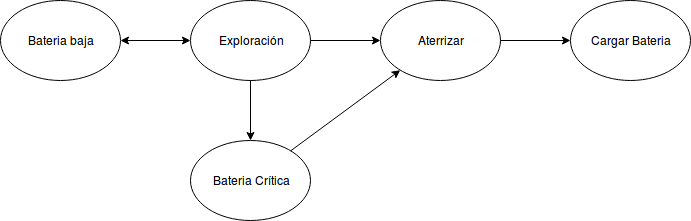
\includegraphics[width=.8\textwidth]{imagenes/chap5/image5}
	\caption{Especificación del estado Bateria.}
\end{figure}

Esta sección de la máquina de estados se encarga de controlar el estado de la batería del dron con el principal objetivo de evitar que el mismo se quede sin carga en la exploración y deba realizar un aterrizaje forzoso sin control del sistema implementado.
Para esto se realiza un chequeo del porcentaje de carga de la  batería y en caso de encontrarse la misma por debajo del 20% se cambia al estado Batería baja. Una vez que el dron se sitúa en este estado el mismo realiza las tareas del estado Exploración descrito anteriormente, con la diferencia de que para determinar la siguiente zona a visitar se consideran como válidas sólo las zonas que se encuentran más cerca de la base con respecto al punto donde se encuentra actualmente, consiguiendo de esta forma reducir en cada movimiento la distancia con respecto a la estación de carga.
A su vez también se realiza un control sobre la distancia entre el dron y la estación de carga y se compara la misma con la cantidad de movimientos necesarios para volver a la estación de carga de forma directa. En caso de que la cantidad de movimientos para volver a la estación de carga sea igual a la cantidad de movimientos restantes más una cantidad predefinida de movimientos se pasa al estado Bateria crítica, donde el dron abandona la exploración y se dirige a la estación de carga. 
Para calcular la distancia a la estación de carga y el camino a seguir se hace uso del algoritmo A*(A aster).
Una vez que el dron llega a la estación de carga pasa al estado Aterrizar, donde se ejecutan las instrucciones para realizar el procedimiento de aterrizaje seguro para más adelante activar el estado Cargar batería. Cuando se termina la carga de la batería el dron vuelve a realizar las tareas de exploración.
\subsection {Coordinación}


\begin{figure}[h!]
	\label{fig:comp}
	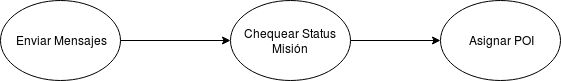
\includegraphics[width=.8\textwidth]{imagenes/chap5/image6}
	\caption{Especificación del estado Coordinación.}
\end{figure}

En esta etapa se realizan las actividades de comunicación de la flota de exploración para optimizar la estrategia a seguir.
Cuando un dron se encuentra en el estado Enviar Mensajes se comunica por medio de la conexión establecida en la Configuración Inicial con los demás miembros de la flota para transmitirle la zona del mapa en la que se encuentra actualmente. De esta forma los demás drones marcan la zona recibida como visitada.
Por otra parte se controla el estado de la vigilancia de los puntos de interés asignadas a otros miembros de la flota, para esto al momento de asignar un punto de interés a un dron se programa una tarea de chequeo a realizar en un período de tiempo preestablecido (el mismo es configurable) cambiando al estado Chequear Status Misión, donde todos los drones disponibles buscan establecer una conexión con el dron que tiene la misión de vigilar la zona asignada. Cuando se recibe una respuesta satisfactoria del dron que se encuentra encargado de la misión se les envía un mensaje a los demás drones para avisarles que la misión está siendo ejecutada con éxito. En caso de que ningún miembro de la flota pueda recibir una respuesta por parte del dron con la misión asignada se determina que la misma fue cancelada y se pasa al estado Asignar POI para reasignar el punto de interés a un nuevo dron disponible.
\subsection {Sin conectividad}


\begin{figure}[h!]
	\label{fig:comp}
	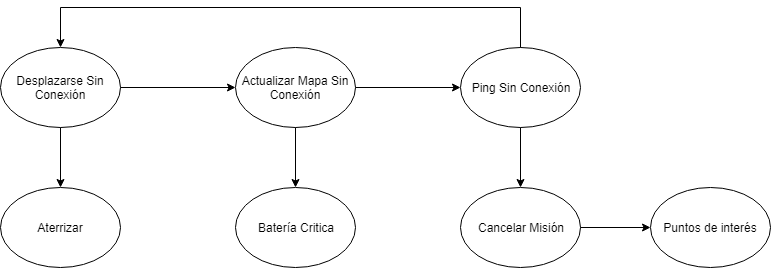
\includegraphics[width=.8\textwidth]{imagenes/chap5/image7}
	\caption{Especificación del estado Sin conectividad.}
\end{figure}

En caso de que el dron no pueda establecer un canal de comunicación con ningún otro miembro de la flota se declara a sí mismo sin conectividad e inicia la ejecución de los estados que se muestran en la Figura 7.
El primer estado en ser ejecutado es Desplazarse Sin Conexión, donde se sigue una estrategia de movimientos similar a la del estado Exploración, con la particularidad de decidir las siguientes zonas a visitar buscando disminuir la distancia con la base, con la finalidad de poder recuperar la conexión con algún dron.
Una vez que el dron haya terminado de desplazarse hacia la nueva zona se cambia el estado a Actualizar Mapa Sin Conexión, donde se actualiza la zona como visitada y se guarda la posición para poder enviarla al resto de la flota en caso de poder restablecer la conexión más adelante.
En el estado Ping Sin Conexión se chequea si se recupero la conexión buscando establecer una comunicación con algún otro dron, en caso de no tener éxito se retorna al estado Desplazarse Sin Conexión, en cambio, si se obtiene una respuesta de otro dron se abandona el modo Sin Conectividad  para volver al funcionamiento habitual.
Si el dron previo a la pérdida de la conectividad tenía asignado un punto de interés se ejecuta el estado Cancelar Misión, donde se enviá un mensaje a los demás drones comunicando que se debe reasignar el punto de interés para posteriormente ejecutar las acciones de Puntos de Interés descritas anteriormente.
En caso de no recuperar la conectividad y llegar a la base se ejecuta el estado Aterrizar para finalizar su ejecución del sistema.
Al igual que cuando se tiene conexión se realiza un control sobre el porcentaje de carga de la batería y se ejecuta el estado Batería Crítica de la misma forma que se describe en la sección Batería.
\subsection {Fin}


\begin{figure}[h!]
	\label{fig:comp}
	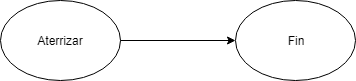
\includegraphics[width=.8\textwidth]{imagenes/chap5/image8}
	\caption{Especificación del estado Fin.}
\end{figure}


Al finalizar la ejecución del sistema se procede al aterrizaje del dron en la base para posteriormente ejecutar el estado Fin donde se cierra el canal de comunicación y se registra la información relevante de la ejecución en archivos con formato csv.
\section{Funcionalidades complementarias}
El sistema desarrollado cuenta con funcionalidades opcionales que se incorporaron en función de considerarse útiles para algunos escenarios de uso particulares.
\subsection{Streaming}
En caso de querer hacer uso del sistema para la vigilancia de un terreno es de gran utilidad poder visualizar desde un centro de control los datos obtenidos por la cámara de los drones.
Por esta razón se incorpora la funcionalidad de poder transmitir en vivo la grabación realizada durante la exploración. Para esto basta con estar conectado a la red wifi en la que se encuentra el dron y recibir los datos enviados por el mismo mediante una conexión UDP en el puerto 4444, estos datos pueden ser visualizados directamente haciendo uso de un reproductor de video (fue verificado con el programa VLC).
Modo de navegación
Al momento de determinar el modo en el que los movimientos de los drones se pueden realizar se analizaron dos alternativas, una que consiste en realizar todos los movimientos sin realizar giros ejecutando desplazamientos de forma lateral en caso de querer moverse hacia un costado, y otra en la que todos los desplazamientos se ejecutan hacia adelante realizando previamente el giro correspondiente.
En función del tiempo necesario para ejecutar los movimientos de rotación se optó por incluir como configuración por defecto no realizar los mismos.
En caso de querer realizar giros en los desplazamientos, lo cual puede resultar útil si se desea activar el streaming de la exploración, es posible activarlo configurando el parámetro correspondiente.

\subsection{Auditoría de la exploración}
Para determinar si la ejecución del sistema cumplió con los objetivos establecidos se incorpora la posibilidad de almacenar en cada dron de la flota de exploración un archivo que contiene estadśiticas detallando el porcentaje de mapa cubierto, la cantidad de puntos de interés visitados y los tiempos de respuesta para las mismas. 
Esta funcionalidad es particularmente útil para la evaluación experimental realizada en la investigación.
\subsection{Altura de vuelo}
Dependiendo de las características del terreno a explorar puede ser necesario configurar a qué altura se debe realizar la exploración. Configurar la altura de vuelo consiste en asignar el rango de altura permitido en metros.
Para determinar la altura a la que se encuentra el dron se utiliza la información publicada por el mismo, la cual hace uso de un sensor para determinar la misma siempre que esta sea menor a 5 metros y cálculos con el GPS para el resto de los casos. 
